\documentclass{beamer}
\usepackage{amsmath}
\usepackage{amsfonts}
\usepackage{mathtools} % for :=
\usepackage{amssymb}
\usepackage{algorithmicx}
\usepackage{algorithm}
\usepackage[noend]{algpseudocode}

\usetheme{Boadilla}
\title{Sparse Distributed Memory for Sparse Rewards}
\subtitle{Honour's Thesis Defense}
\author{Alex Van de Kleut}
\institute{Brock University}
\date{\today}

\begin{document}
\begin{frame}
  \titlepage
\end{frame}

\begin{frame}
  \frametitle{Reinforcement Learning}
  Context:
  \begin{itemize}
    \item Agent
    \item Environment
    \item $\langle s_t, a_t, r_t, s_{t+1} \rangle$
  \end{itemize}
  \begin{figure}
    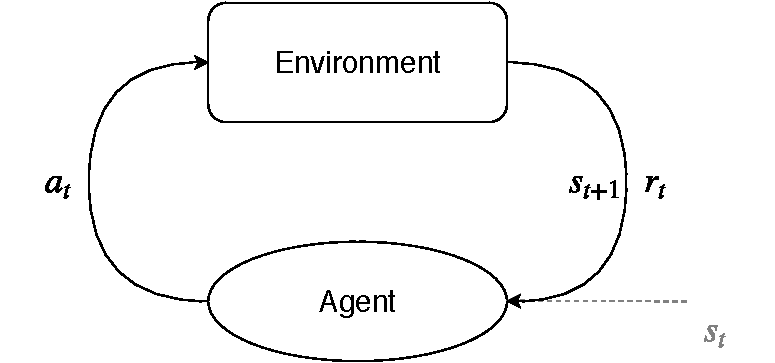
\includegraphics[scale=0.5]{assets/rl.pdf}
  \end{figure}
\end{frame}

\begin{frame}
  \frametitle{Markov Decision Process}
  \begin{itemize}
    \item $\left( \mathcal{S}, \mathcal{A}, \mathcal{P}, \mathcal{R} \right)$
    \item $\mathcal{P}(s_t, a_t, s_{t+1}) = \mathbb{P} \left[ s_{t+1} \vert s_t, a_t\right]$
    \item $\mathcal{R}(s_t, a_t) = \mathbb{E} \left[ r_t \vert s_t, a_t \right]$
  \end{itemize}
  \begin{figure}
    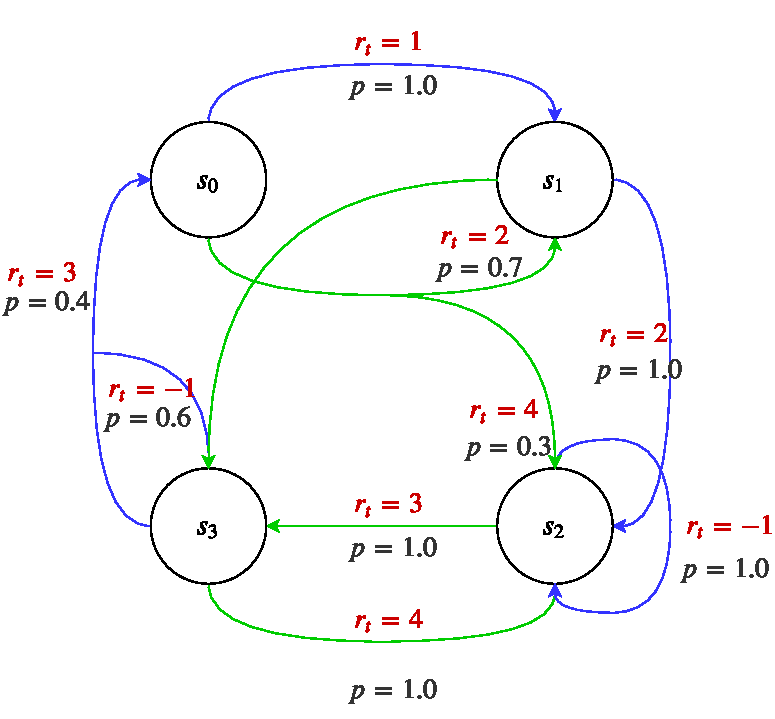
\includegraphics[scale=0.5]{assets/mdp.pdf}
  \end{figure}
\end{frame}

\begin{frame}
  \frametitle{Trajectories, Returns, Policies}
  \begin{itemize}
    \item Trajectory: $\tau = \langle s_0, a_0, r_0, s_1, a_1, r_1, \dots \rangle$
    \item Return:
    \begin{itemize}
      \item $R_t = \sum_{k=t}^\infty r_k$
      \begin{itemize}
        \item Not guaranteed to converge
      \end{itemize}
      \item $G_t = \sum_{k=t}^\infty \gamma^{t-k}r_k$
      \begin{itemize}
        \item Guaranteed to converge
      \end{itemize}
    \end{itemize}
    \item Policy: $\pi : \mathbb{P} \left[ a_t \vert s_t \right]$
      \begin{block}{The Reward Hypothesis}
        Every action of a rational agent can be thought of as seeking to maximize some cumulative reward signal.
      \end{block}
      \begin{exampleblock}{Goal}
        Learn a policy $\pi$ that chooses actions $a \sim \pi(\cdot \vert s_t)$ that maximize $G_t$
      \end{exampleblock}
  \end{itemize}
\end{frame}

\begin{frame}
  \frametitle{Value, Quality, $Q$-learning}
  \begin{block}{Value}$$V^\pi(s_t) = \mathbb{E}_\pi \left[ G_t \vert s_t \right] = \mathbb{E}_\pi \left[ r_t + \gamma V^\pi(s_{t+1}) \vert s_t \right]$$
  \end{block}
  \begin{block}{Quality}
  $$Q^\pi(s_t, a_t) = \mathbb{E}_\pi \left[ G_t \vert s_t, a_t \right] = \mathbb{E}_\pi \left[ r_t + \gamma Q^\pi(s_{t+1}, a_{t+1}) \vert s_t, a_t \right]$$
\end{block}
  In practice, $V^\pi$ and $Q^\pi$ are unknowable, so we approximate it with some functions $V$ and $Q$.
\begin{exampleblock}{Q-learning}
  \begin{equation*}
    \pi(a_t \vert a_t) = \begin{cases} 1 & a_t = \arg \max_{a_t} Q(s_t, a_t) \\ 0 & \text{otherwise} \end{cases}
  \end{equation*}
  \begin{equation*}
    Q(s_t, a_t) \gets Q(s_t, a_t) + \alpha(r_t + \gamma \max_{a_{t+1}} Q(s_{t+1}, a_{t+1}) - Q(s_t, a_t))
  \end{equation*}
\end{exampleblock}
\end{frame}

\begin{frame}
  \frametitle{Deep $Q$-learning}
  \begin{itemize}
    \item It is unfeasible to store $Q(s_t, a_t)$ when $\mathcal{S}$ is large or infinite.
    \item Instead, we use a neural network $Q_\theta$ as a function approximator for $Q$
    \item Produces a vectorized output for predicted $Q$ over each action
    \begin{itemize}
      \item Requires discrete $\mathcal{A}$
    \end{itemize}
    \item $Q$-network minimizes prediction error between $Q_\theta(s_t, a_t)$ and $r_t + \gamma Q_\theta(s_{t+1}, a_{t+1})$ using \textbf{gradient descent}:
  \end{itemize}
  \begin{exampleblock}{Deep $Q$-learning}
    \begin{equation*}
          L(\theta) = \mathbb{E}_{a_t \sim \pi} \left[ \left(y_i - Q_\theta(s_t, a_t) \right)^2 \right]
    \end{equation*}
    \begin{equation*}
      y_i = \mathbb{E}_{a_{t+1} \sim \pi} \left[ r_t + \gamma \max_{a_{t+1}} Q_\theta (s_{t+1}, a_{t+1}) \vert s_t, a_t \right]
    \end{equation*}
    \begin{equation*}
      \theta \gets \theta - \frac{1}{2} \alpha \nabla_\theta L(\theta)
    \end{equation*}
  \end{exampleblock}
\end{frame}

\begin{frame}
  \frametitle{Policy Gradient}
  \begin{itemize}
    \item Deep $Q$-learning uses discrete $\mathcal{A}$ and uses a greedy policy.
    \item Policy gradients model the policy using a set of parameters $\theta$
    \item Policy gradients directly optimize the policy, allow for stochastic policies, and allow continuous action spaces.
  \end{itemize}
  \begin{equation}
    \pi_\theta (a_t \vert s_t) = \mathbb{P} \left[a_t \vert s_t; \theta \right]
  \end{equation}
  \begin{block}{Softmax Distribution}
    Output mapped to probability distribution
    \begin{equation*}
      a_i \to \frac{e^{a_i}}{\sum_j e^{a_j}}
    \end{equation*}
  \end{block}
  \begin{block}{Diagonal Gaussian Distribution}
    Output treated as mean of continuous action space
    \begin{equation*}
      a_t = \mu_\theta(s_t) + z \odot \sigma
    \end{equation*}
  \end{block}
\end{frame}
\begin{frame}
\frametitle{Policy Gradient Theorem}
  We define an objective function $J(\theta)$ that we want our policy to maximize. If $\pi_\theta$ is differentiable, we can use \textbf{gradient ascent}:
  \begin{exampleblock}{Policy Gradient Theorem}
    \begin{equation}
      \theta \gets \theta + \alpha \nabla_\theta J(\theta)
    \end{equation}
    \begin{equation*}
      \nabla_\theta J(\theta) = \mathbb{E}_{\pi_\theta} \left[ \nabla_\theta \log \pi_\theta (a_t \vert s_t) Q^{\pi_\theta}(s_t, a_t) \right]
    \end{equation*}
  \end{exampleblock}
  Full derivation in thesis.
\end{frame}

\begin{frame}
  \frametitle{REINFORCE, Actor-Critic}
  \begin{block}{REINFORCE}
    Since policy gradient theorem is an expectation, we can sample this estimation to get approximate the gradient.
    \begin{equation*}
    \theta \gets \theta + \alpha \nabla_\theta \log \pi_\theta (a_t \vert s_t) G_t
    \end{equation*}
  \end{block}
  \begin{block}{Actor-Critic}
    Monte-carlo methods like REINFORCE subject to high variance.
    \begin{itemize}
      \item Actor: The policy $\pi_\theta$
      \item Critic: A deep neural network $\mathcal{S} \to \mathbb{R}$ that learns to approximate $V(s_t)$ in a manner analogous to deep $Q$-learning.
    \end{itemize}
  \end{block}
\end{frame}

\begin{frame}
  \frametitle{Advantage, Generalized Advantage Estimation}
  The $Q^{\pi_\theta}$ term in the policy gradient can have high variance. We can subtract a baseline $b(s)$ without changing the expectation.
  \begin{block}{Advantage}
    \begin{equation*}
      A^{\pi_\theta}(s_t, a_t) = Q^{\pi_\theta}(s_t, a_t) - V^{\pi_\theta}(s_t)
    \end{equation*}
  \end{block}
  \begin{exampleblock}{Generalized Advantage Estimation}
    \begin{align*}
        \hat{A}_t = \sum_{i=0}^\infty (\gamma \lambda)^i \delta_{t+i}^{\pi_\theta}
        & &
        \delta_t^{\pi_\theta} = r_t + \gamma V^{\pi_\theta} (s_{t+1}) - V^{\pi_\theta}(s_t)
    \end{align*}
    rather than two sets of parameters to approximate $Q^{\pi_\theta}(s_t, a_t)$ and $V^{\pi_\theta}(s_t)$, we use one: $V_\phi$. Then $V_\phi$ we update $\phi$ to minimize $$d_t(\phi) = r_t + \gamma V_\phi(s_{t+1}) - V_\phi(s_t)$$ and update $\theta$ to maximize $\hat{A}_t$.
  \end{exampleblock}
\end{frame}

\begin{frame}
  \frametitle{Proximal Policy Optimization (PPO)}
  \begin{alertblock}{PPO}
    Modified objective function based on direction of policy updates.
    \begin{equation*}
      J(\theta) = \mathbb{E}_{\pi_\theta} \left[ \rho(\theta) A^{\pi_\theta}(s, a) \right]
    \end{equation*}
    where
    \begin{equation*}
      \rho(\theta) = \frac{\pi_\theta (a \vert s)}{\pi_{\theta_\text{old}} (a \vert s)}
    \end{equation*}
  \end{alertblock}
  When $\rho(\theta) > 1$ then we increased the likelihood of $\pi_\theta(a_t \vert s_t)$.
  \begin{table}
  \begin{tabular}{|c|cc|}
    \hline
    & $\rho(\theta) > 1$ & $\rho(\theta) < 1$ \\ \hline
    $A^{\pi_\theta}(s, a) > 0$ & Good (clip) & Bad (roll back) \\
    $A^{\pi_\theta}(s, a) < 0$ & Bad (roll back) & Good (clip) \\ \hline
  \end{tabular}
\end{table}
\begin{itemize}
  \item Clipping means policy updates are conservative
  \item Allows us to do multiple epochs of policy updates on same batch of training experience (faster learning)
\end{itemize}
\end{frame}

\begin{frame}
  \frametitle{Sparse Rewards}
  \begin{itemize}
    \item RL works best when rewards are \textbf{dense} (mostly nonzero).
    \item RL struggles when rewards are \textbf{sparse}
    \item Requires \textbf{intrinsic motivation} - method for agent to reward itself
    \begin{itemize}
      \item What is rational behaviour without a clear goal?
      \item Exploration, curiosity, etc.
      \item Design intrinsic reward to encourage these behaviours to increase likelihood of finding sparse extrinsic rewards.
    \end{itemize}
  \end{itemize}
  \begin{exampleblock}{Count-Based}
    Methods for keeping track of how often certain states have been visited, with reward inversely proportional to visitation frequency.
  \end{exampleblock}
  \begin{exampleblock}{Forward-Dynamics}
    Try to predict next state given current state and action, with reward proportional to prediction error. Subject to noisy tv problem.
  \end{exampleblock}
\end{frame}

\begin{frame}
  \frametitle{Random Network Distillation}
  Novel approach to intrinsic motivation that achieves state-of-the-art performance on Montezuma's Revenge, a sparse reward environment.
  \begin{columns}
    \column{0.5\textwidth}
    \begin{alertblock}{RND}
      Two neural networks
      \begin{itemize}
        \item Feature network: $\mathcal{S} \to \mathbb{R}^k$
        \item Predictor network: same architecture as feature network with different initialization. Learns to predict output of feature network.
      \end{itemize}
      Commonly visited state will have lower prediction error. Reward proportional to prediction error.
    \end{alertblock}
    Poor sample efficiency! Takes $1.6 \times 10^9$ frames to achieve SOTA performance.
    \column{0.5\textwidth}
    \begin{figure}
      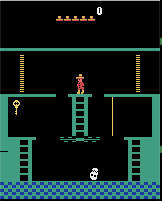
\includegraphics{assets/mr.png}
    \end{figure}
  \end{columns}
\end{frame}

\begin{frame}
  \frametitle{Sparse Distributed Memory}
  How can we have an intrinsic reward signal like RND that works immediately?
  \begin{columns}
    \column{0.4\textwidth}
    \begin{alertblock}{SDM}
      \begin{itemize}
        \item Computer memory for long ($>100$-bit) words
        \item Small subset of address space implemented in hardware
        \item Reading and writing distributed to addresses `close' to the one specified
        \item \textbf{autoassociative memory}
      \end{itemize}
    \end{alertblock}
    \column{0.6\textwidth}
    \begin{figure}
      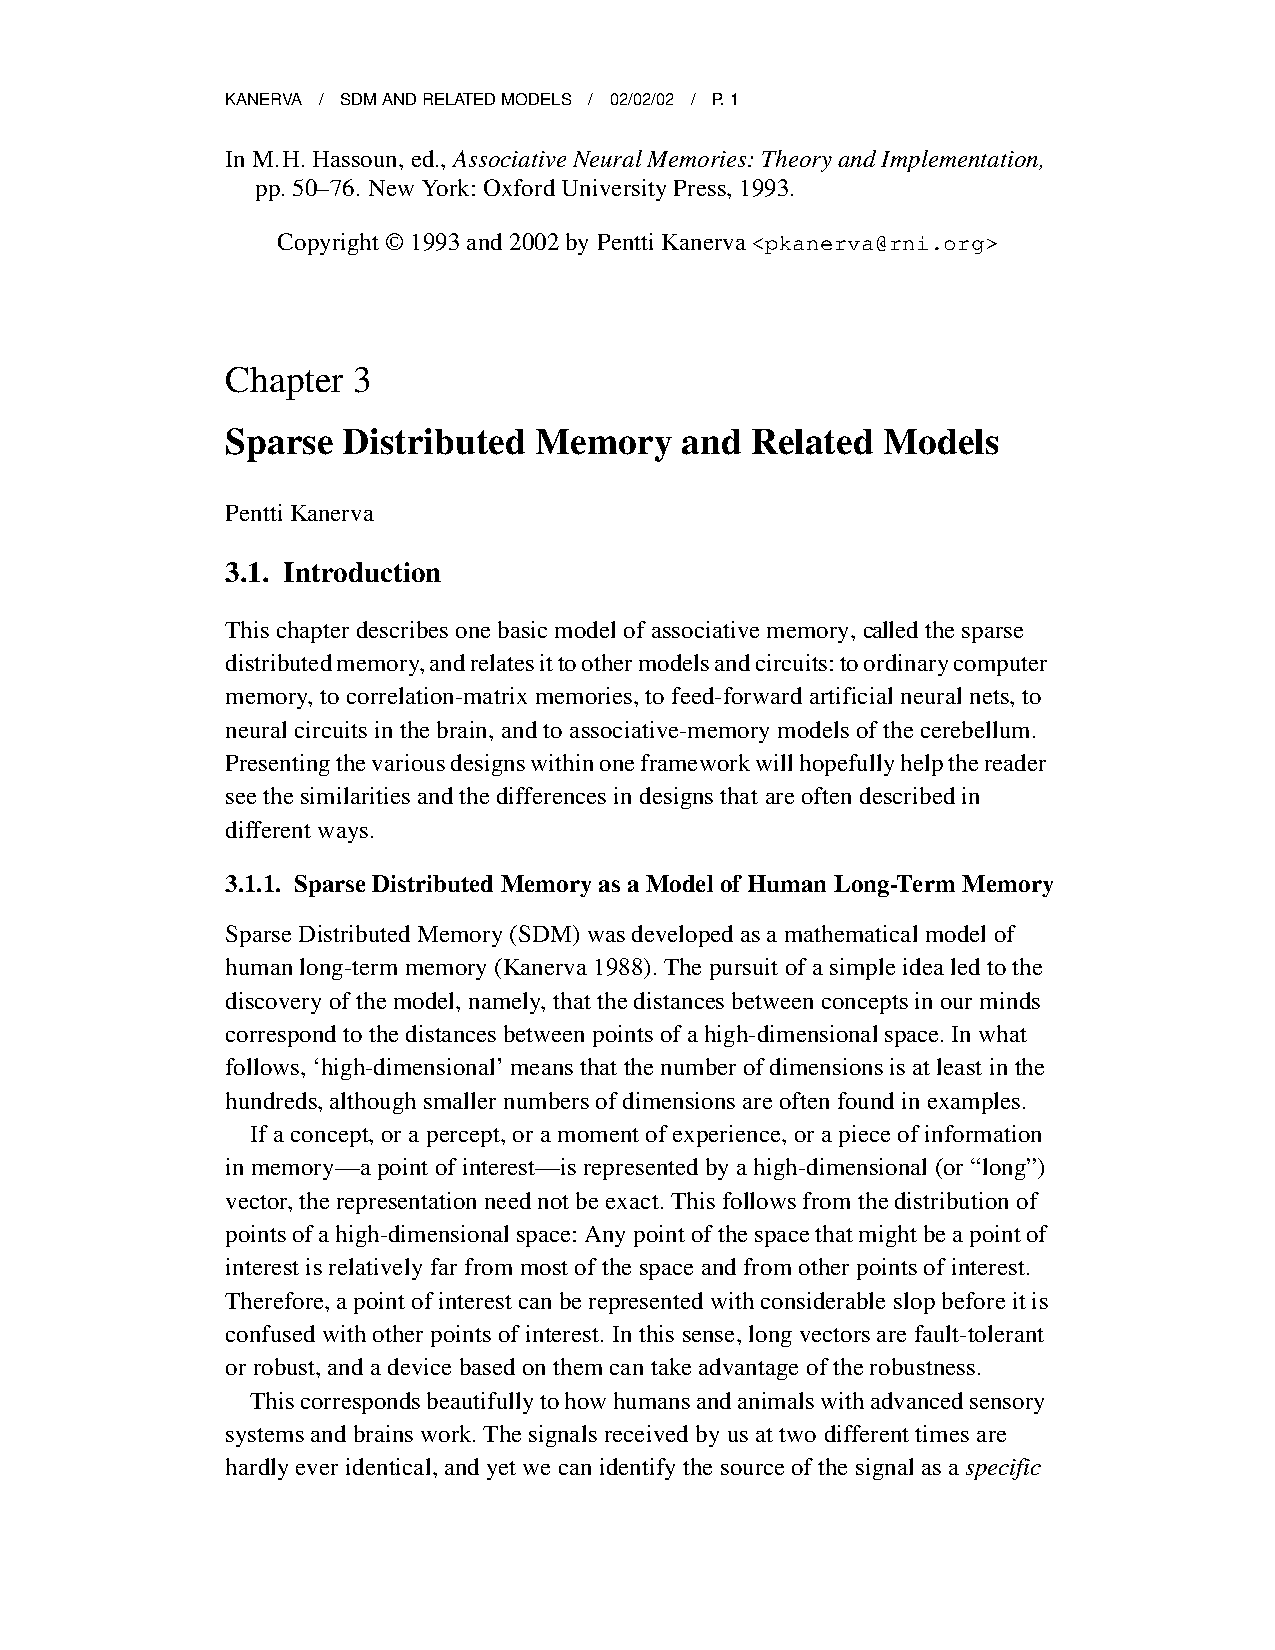
\includegraphics[scale=0.25]{assets/sdm.png}
    \end{figure}
  \end{columns}
\end{frame}

\begin{frame}
  \frametitle{Hashing}

  \begin{columns}
    \column{0.5\textwidth}
      Data written to/read from memory is hashed state: $\text{Hash}: \mathcal{S} \to \{ 0, 1 \}^N$
      \begin{itemize}
        \item We want hashes for similar states to be similar.
        \item We can use a neural network with the same architecture as the feature network from RND.
        \item If that network's output is $o$, then we can define the following hash:
      \end{itemize}
      \begin{exampleblock}{}
        \begin{equation}
          \text{Hash}(s_t)_i = \begin{cases} 1, & o_i \geq \bar{o} \\ 0, & o_i < \bar{o} \end{cases}
        \end{equation}
      \end{exampleblock}
      \column{0.5\textwidth}
      \begin{figure}
        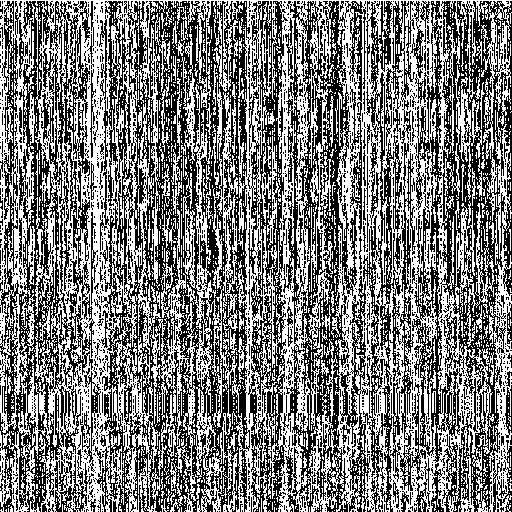
\includegraphics[scale=0.25]{assets/hashes.jpg}
      \end{figure}
  \end{columns}
\end{frame}

\begin{frame}
  \frametitle{Proof of Concept}
  \begin{columns}
    \column{0.5\textwidth}
    \begin{itemize}
      \item Agent is in state $s_t$ and computes a hash $\mathbf{w}_t$ of the state
      \item Agent checks memory at address $\mathbf{w}_t$ and retrieves stored binary vector $\mathbf{z}_t$
      \item Agent computes intrinsic reward by taking scaled hamming distance between $\mathbf{w}_t$ and $\mathbf{z}_t$
      \item Agent stores $\mathbf{w}_t$ to memory
    \end{itemize}
    \begin{exampleblock}{}
      \begin{equation*}
        r_t^I = \frac{d_H(\mathbf{w}_t, \mathbf{z}_t)}{N}
      \end{equation*}
    \end{exampleblock}
    \column{0.5\textwidth}
    \begin{figure}
      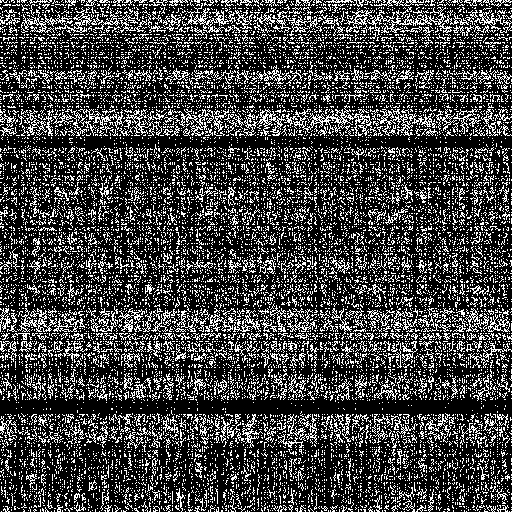
\includegraphics[scale=0.25]{assets/xor-diffs.jpg}
    \end{figure}
  \end{columns}
\end{frame}

\begin{frame}[shrink]
  \frametitle{Pseudocode}
	\begin{algorithmic}
		\State $N \gets$ number of rollouts
		\State $N_\text{opt} \gets$ number of optimization epochs
		\State $K \gets$ length of rollout
		\State $t = 0$
		\State sample $s_0$ from $d(s)$
		\For {$i = 1$ to $N$}:
			\For {$j = 1$ to $K$}:
				\State sample $a_t \sim \pi_\theta(s_t)$
				\State sample $s_{t+1}, r_t^E$ from $\mathcal{P}, \mathcal{R}$
				\State normalize state $s_t \gets \frac{s_t - \mu}{\sigma}$
				\State compute $\mathbf{w} = \text{Hash}(s_t)$
				\State compute intrinsic reward $r_t^I$
				\State normalize intrinsic reward
				\State store $s_t, a_t, r_t^E, r_t^I$ to optimization batch $B_i$
				\State $t = t+1$
			\EndFor
			\State compute $A_E$ and $A_I$ for batch $B_i$ using GAE
			\State compute total advantage $A = c_E A_E + c_I A_I$
			\For {$j = 1$ to $N_\text{opt}$}:
				\State optimize policy using PPO
			\EndFor
		\EndFor
	\end{algorithmic}
\end{frame}

\begin{frame}
  \frametitle{Results}
  \begin{figure}
    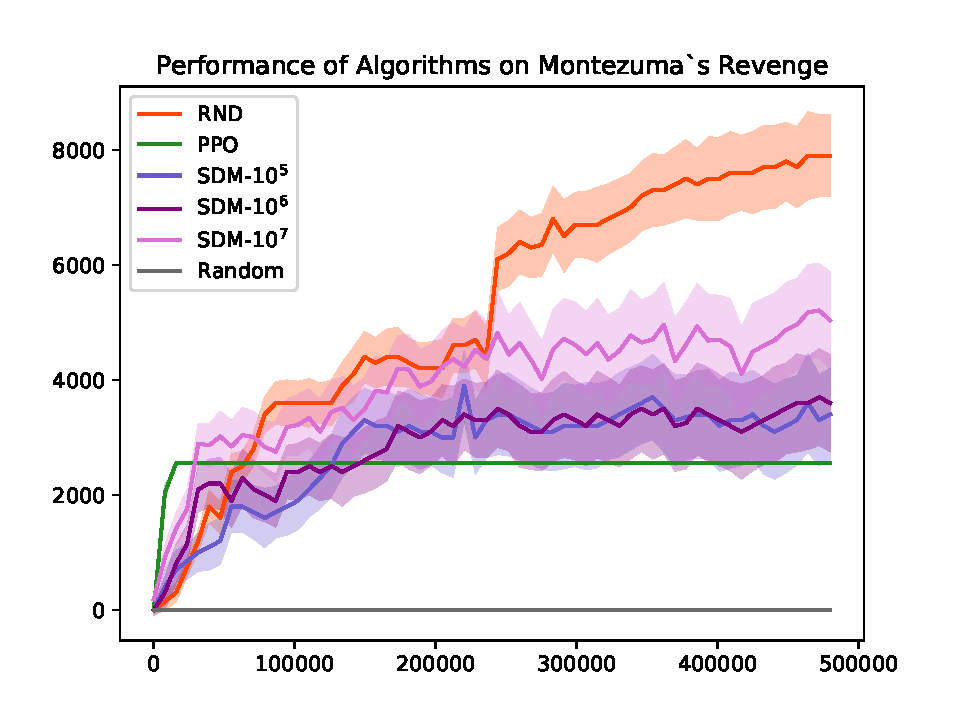
\includegraphics[scale=0.4]{assets/training-curve.pdf}
  \end{figure}
  \begin{table}
    \tiny
  \begin{tabular}{c |c c c c}
    $M$ & Cumulative Reward & RND-Normalized & PPO-Normalized & Random-Normalized \\ \hline
    $10^5$ & $3607 \pm 651$ & $45.82\%$ & $141.45\%$ & $13035\%$\\
    $10^6$ & $3553 \pm 428$ & $45.15\%$ & $139.33\%$ & $17765\%$\\
    $10^7$ & $4251 \pm 399$ & $54.01\%$ & $166.71\%$ & $21255\%$\\
    \hline
    RND & $7871 \pm 676$ & & & \\
    PPO & $2550 \pm 0$ & & & \\
    Random & $20 \pm 40$ & & & \\

  \end{tabular}
\end{table}
\end{frame}

\begin{frame}
  \frametitle{Results}
  \begin{itemize}
    \item SDM improves performance over PPO baselines (significant improvement, $p<0.05$)
    \item SDM competitive with RND up to around halfway through training
    \begin{itemize}
      \item RND finds room with easy access to many other rooms
    \end{itemize}
    \item Some increase in performance associated with increasing memory size to $M=10^7$
    \item All methods perform significantly better than random
    \item Overall: SDM plays at amateur human level
  \end{itemize}
\end{frame}

\begin{frame}
  \frametitle{Discussion}
  \begin{itemize}
    \item SDM improvement over PPO demonstrates that using intrinsic reward can improve exploration and increase likelihood of finding sparse extrinsic rewards
    \item Rate at which intrinsic reward dissipates is much faster for SDM than for RND
    \begin{itemize}
      \item Originally the motivation for this technique, actually hampered the agent's learning
      \item Intrinsic rewards become sparse quickly for common states
      \item No extrinsic \textit{or} intrinsic rewards
    \end{itemize}
    \item Intrinsic reward disappears completely around $300,000$ parameter updates: agent is learning using only PPO at this point
  \end{itemize}
\end{frame}

\begin{frame}
  \frametitle{Future Work}
  \begin{enumerate}
    \item Compare RND to SDM in a complex state space (such as a 3D environment)
    \begin{itemize}
      \item Possible that RND networks take too long to learn since inputs vary significantly more than with Montezuma's Revenge
      \item Instanteneity of SDM becomes more important here
    \end{itemize}
    \item Write schedule that writes only when states are novel rather than every time step
    \begin{itemize}
      \item Reduce rate of reward evaporation
    \end{itemize}
    \item Used a discrete action space environment here:
    \begin{itemize}
      \item Extend intrinsic reward methods to deep $Q$-learning rather than just policy gradient methods?
    \end{itemize}
  \end{enumerate}
\end{frame}

\begin{frame}[shrink]
  \frametitle{Conclusion}
  \begin{columns}
    \column{0.25\textwidth}
    \begin{itemize}
      \small
      \item Reinforcement learning struggles when rewards are sparse
      \item SDM improves performance in Montezuma's Revenge over baseline performance by introducing memory-based intrinsic reward
      \item SDM's performance does not achieve state-of-the-art
    \end{itemize}
    \column{0.75\textwidth}
    \begin{figure}
      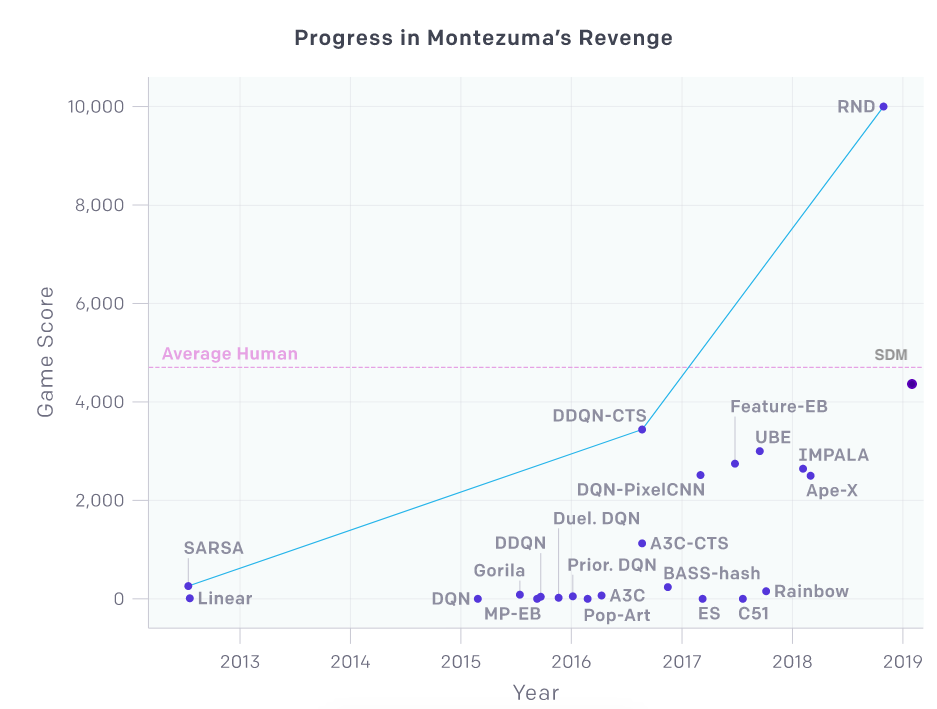
\includegraphics[scale=0.25]{assets/progress.png}
    \end{figure}
  \end{columns}
\end{frame}

\end{document}
